\documentclass[10pt]{beamer}

% mac版,texShop 中Typeset选择 XeLaTex 

%%%%%%%%%%%%%%%%%%%%%%%%%%%%%%%%%%%%%
\usepackage[slantfont,boldfont]{xeCJK}
%\input{xecjkfonts},CJKtextspaces
\setCJKmainfont{STKaiti}   % STFangsong 设置缺省中文字体
\setCJKmonofont{SimSun}   % 设置等宽字体
\setmainfont{Times} % 英文衬线字体
\setmonofont{Times} % 英文等宽字体
\setsansfont{Times} % 英文无衬线字体
%%%%%%%%%%%%%%%%%%%%%%%%%%%%%%%%%%%%%%

\mode<presentation> {
  %\usetheme{Madrid}
  %\usetheme{Singapore}
  \usetheme{Warsaw}
  \setbeamercovered{transparent}
 % \usefonttheme[onlymath]{serif}  
 \usefonttheme{professionalfonts}%{structurebold}
 % \usefonttheme[onlymath]{structurebold}
  \usecolortheme{rose}
}

\usepackage[english]{babel}
%\usepackage[latin1]{inputenc}

%\usepackage{times}
%\usepackage[T1]{fontenc}


%\usepackage{epsfig}
\usepackage{graphics}
\usepackage{color}
\usepackage{amsmath,amssymb,mathrsfs}
\usepackage{amsfonts,stmaryrd}
%\usepackage{thmmarks}
%\usepackage{}



\newcommand\frakfamily{\usefont{U}{yfrak}{m}{n}}
\DeclareTextFontCommand{\textfrak}{\frakfamily}
\def\diag{\mathrm{diag}}


\title[数值计算方法]{数值计算方法}
\subtitle{-数值计算方法理论选讲:适定性与条件数}


\subject{Talks}

% If you have a file called "university-logo-filename.xxx", where xxx
% is a graphic format that can be processed by latex or pdflatex,
% resp., then you can add a logo as follows:

% \pgfdeclareimage[height=0.5cm]{university-logo}{university-logo-filename}
% \logo{\pgfuseimage{university-logo}}

%\pgfdeclareimage[height=0.5cm]{university-logo}{ncsu_logo}
%\logo{\pgfuseimage{university-logo}}

% Delete this, if you do not want the table of contents to pop up at
% the beginning of each subsection:
%\AtBeginSubsection[] {
%  \begin{frame}<beamer>
%    \frametitle{Outline}
%    \tableofcontents[currentsection,currentsubsection]
%  \end{frame}
%}

% If you wish to uncover everything in a step-wise fashion, uncomment
% the following command:

% \beamerdefaultoverlayspecification{<+->}


\setbeamertemplate{theorems}[numbered]
\setbeamertemplate{caption}[numbered]


\newtheorem{proposition}[theorem]{Proposition}

%%%%%%%%%%%%%%%%%%%%%%%%%%%
% REMARK-STYLE-ENVIRONMENTS %
%%%%%%%%%%%%%%%%%%%%%%%%%%%
\newcounter{remark}
% \numberwithin{theorem}{section}
\def\openrem#1#2{\refstepcounter{remark}\bigskip

{\noindent\bf#1~\theremark\if#2!{. }\else{ (#2).}\fi}
\it}
\def\thmskip{}
\newenvironment{remark}[1][!]{\openrem{Remark}{#1}}{\thmskip}

%%%%%%%%%%%%%%%%%%%%%%%%%%%%
%% AlGORITHM-STYLE-ENVIRONMENTS %
%%%%%%%%%%%%%%%%%%%%%%%%%%%%
\newcounter{algorithm}
% \numberwithin{theorem}{section}
\def\openalg#1#2{\refstepcounter{algorithm}\bigskip

{\noindent\bf#1~\thealgorithm\if#2!{. }\else{ (#2).}\fi}
\it}
\def\thmskip{}
\newenvironment{algorithm}[1][!]{\openrem{Algorithm}{#1}}{\thmskip}
%
%
%%%%%%%%%%%%%%%%%%%%%%%%%%%%
%% Result-STYLE-ENVIRONMENTS %
%%%%%%%%%%%%%%%%%%%%%%%%%%%%
%\newcounter{result}
%\def\openrem#1#2{\refstepcounter{result}\bigskip
%{\noindent \it \bfseries#1~\theremark\if#2!{. }\else{ (#2). }\fi}}
%\newenvironment{result}[1][!]{\openrem{Result}{#1}}{\qed}




%%%%%%%%%%%%%%%%%%%%%%%%%%%
%Redefine the Symbols%
%%%%%%%%%%%%%%%%%%%%%%%%%%%

\def\mathbi#1{\textbf{\em #1}}

% integrals
\def\dx{\,{\rm d}x}
\def\dxb{\,{\rm d}\boldsymbol{x}}
\def\dy{\,{\rm d}y}
\def\dt{\,{\rm d}t}
\def\ds{\,{\rm d}s}
\def\du{\,{\rm d}u}

\def\dr{\,{\rm d}r}
\def\dtheta{\,{\rm d}\theta}

\def\dd{{\rm d}}

\def\intOm{\int_{\Omega}}
\def\intbOm{\int_{\partial \Omega}}

% differences
\def\Dx{\Delta x}
\def\Dt{\Delta t}
\def\D{\Delta}


% operators
\def\Ls{\mathscr{L}}

% matirices
\def\Js{\mathscr{J}}


%fields%
\def\R{\mathbb{R}}
\def\N{\mathbb{N}}
\def\Z{\mathbb{Z}}

%Spaces%
\def\H{\mathbb{H}}
\def\L{\mathbb{L}}
\def\P{\mathbb{P}}


\def\U{\mathbb{U}}
\def\V{\mathbb{V}}
\def\W{\mathbb{W}}
\def\X{\mathbb{X}}
\def\Y{\mathbb{Y}}

\def\Cinfty{C^\infty}




%vectors%
\def\ab{\boldsymbol{a}}
\def\bb{\boldsymbol{b}}
\def\cb{\boldsymbol{c}}
\def\db{\boldsymbol{d}}
\def\eb{\boldsymbol{e}}
\def\fb{\boldsymbol{f}}
\def\gb{\boldsymbol{g}}
\def\hb{\boldsymbol{h}}
\def\nb{\boldsymbol{n}}
\def\rb{\boldsymbol{r}}
\def\sb{\boldsymbol{s}}


\def\ub{\boldsymbol{u}}
\def\vb{\boldsymbol{v}}
\def\wb{\boldsymbol{w}}
\def\xb{\boldsymbol{x}}
\def\yb{\boldsymbol{y}}
\def\zb{\boldsymbol{z}}

\def\Bb{\boldsymbol{B}}
\def\Cb{\boldsymbol{C}}
\def\Eb{\boldsymbol{E}}
\def\Fb{\boldsymbol{F}}
\def\Ib{\boldsymbol{I}}
\def\Kb{\boldsymbol{K}}
\def\Ob{\boldsymbol{O}}
\def\Qb{\boldsymbol{Q}}
\def\Rb{\boldsymbol{R}}
\def\Sb{\boldsymbol{S}}
\def\Ub{\boldsymbol{U}}
\def\Vb{\boldsymbol{V}}
\def\Wb{\boldsymbol{W}}
\def\Xb{\boldsymbol{X}}
\def\Yb{\boldsymbol{Y}}
\def\Zb{\boldsymbol{Z}}

%domains%
\def\Om{\Omega}
\def\bd{\partial}
\def\bOm{\bar{\Omega}}

%bold symbols%
\def\alphab{\boldsymbol{\alpha}}
\def\phib{\boldsymbol{\varphi}}

%energy%
\def\Jc{\mathcal{J}}
\def\Oc{\mathcal{O}}

%Greeks%
\def\vphi{\varphi}

%Special Functions%
\def\supp{\rm{supp}}
\def\sym{\rm{sym}}

\def\gradu{\nabla u}
\def\gradv{\nabla v}

%Mesh%
\def\Ts{\mathcal{T}}

\def\mach{\rm{mach}}


\begin{document}

\setbeamertemplate{itemize item}[triangle]

\begin{frame}
\titlepage
\end{frame}


\begin{frame}
  \frametitle{本节概要}
  \tableofcontents%[pausesections]
  % You might wish to add the option [pausesections]
%  \begin{itemize}
%  \item 显示Euler法及其误差分析
%  \item Taylor展开法
%  \item 
%  \end{itemize}
\end{frame}

\section{向前与向后误差}

\begin{frame}
\frametitle{求根运算的误差}
首先看一个例子
\begin{example}
利用二分法求$f(x) = x^3 - 2x^2 + \frac{4}{3}x - \frac{8}{27}$的根,精确到6位有效数字。
\end{example}
首先注意到$f(0)f(1) = -\frac{8}{27}\frac{1}{27} <0$,所以在$[0,1]$上一定有一个根。根据二分法的误差估计,$20$步的二分可以使结果具有6位有效数字。

\vspace{0.1cm}

另一方面容易得到
\begin{equation}
f(\frac{2}{3}) = \frac{8}{27} - 2\frac{4}{9} + \frac{4}{3} \frac{2}{3} - \frac{8}{27} = 0,
\end{equation}
即$\frac{2}{3}$是原方程在$[0,1]$上的一个根。
\end{frame}


\begin{frame}
\frametitle{求根运算的误差}
那么如果用二分法进行求根,事实上会得到什么结果呢?可以见下表
\begin{figure}
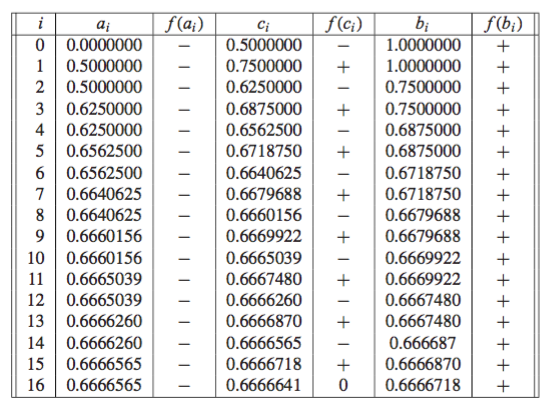
\includegraphics[width=8cm]{figs/1-3-1_Foward&Backward_Error-1} 
%\caption{$f(x) = x^3 + x -1$的图像} 
\end{figure}
程序在第16步就停止了,停止的原因是计算机的计算结果显示$f(0.6666641)=0$。
\end{frame}


\begin{frame}
\frametitle{求根运算的误差}
如果我们对结果的精度要求比较高的话,那么上面的计算实际上是失败了。但是只要我们使用IEEE双精度进行计算,那么在$r = \frac{2}{3}$的$10^{-5}$的邻域内有很多双精度数使得$f(x)=0$,换句话说,有很多数可以称为$f(x)= 0$的根。更严重的是,虽然$f(x)$是一个单调递增的函数,但是在双精度浮点运算中$f(x)$并不是单调递增的,可以见下图
\begin{figure}
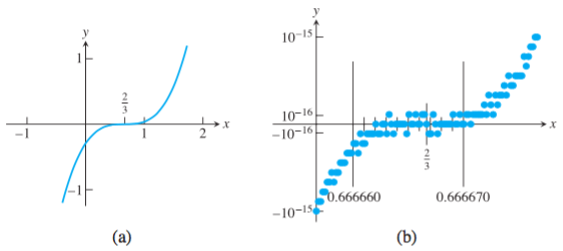
\includegraphics[width=8cm]{figs/1-3-1_Foward&Backward_Error-2} 
%\caption{$f(x) = x^3 + x -1$的图像} 
\end{figure}
事实上,我们无法得到精确度足够高的解的原因并不在于二分法这种数值方法,而在于双精度浮点运算无法精确计算$f(x)$在根$r = \frac{2}{3}$附近的值。
\end{frame}


\begin{frame}
\frametitle{向前与向后误差}
\begin{definition}[向前向后误差]
设$r$是$f(x) = 0$的根。假设$x_a$是$r$的一个近似,那么对于数值求根问题,近似值$x_a$的向后误差是$|f(x_a)|$,而$x_a$的向前误差是$|r - x_a|$。
\end{definition}

这里我们对向前和向后误差作一些解释。我们将问题抽象为这样一个过程
\begin{figure}
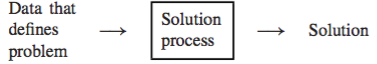
\includegraphics[width=6cm]{figs/1-3-1_Foward&Backward_Error-3} 
%\caption{$f(x) = x^3 + x -1$的图像} 
\end{figure}
或者特别的对于求解方程我们抽象为
\begin{figure}
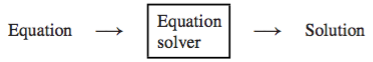
\includegraphics[width=6cm]{figs/1-3-1_Foward&Backward_Error-4} 
%\caption{$f(x) = x^3 + x -1$的图像} 
\end{figure}
\end{frame}


\begin{frame}
\frametitle{向前与向后误差(Backward and Forward Error)}
如果我们以求解过程为所在地,按照箭头的指向站立,那么向后看就是问题的输入,而向前看就是问题的输出。
所以在问题输入端的误差被称为向后误差,而问题输出端的误差就是向前误差。

\vspace{0.2cm}

对于求解方程,我们可以这样理解:
\begin{itemize}
\item 问题的输入相当于是$f(x)$的值,误差相当于是我们需要对$f(x)$的值作多大的调整才能使得$x_a$是方程的解。这个调整值当然是$|f(x_a)|$,即$x_a$是方程$f(x) - f(x_a) = 0$的解。(输出端不动,改变输入端使(新的)方程成立)
\item 问题的输出相当于是$x_a$,误差相当于是我们需要对$x_a$的值作多大的调整才能满足方程$f(x) = 0$。这个调整当然是$|r - x_a|$,即$f(r) = 0$。(输入端不动,改变输出端使方程成立)
\end{itemize}
\end{frame}


\begin{frame}
\frametitle{向前与向后误差(Backward and Forward Error)}
之前的例子当中,我们遇到的困难是
\begin{equation}
\text{向后误差} \approx \epsilon_{mach} \approx 2.2 \times 10^{-16}.
\end{equation}
而与此同时
\begin{equation}
\text{向前误差} \approx 10^{-5}.
\end{equation}
由于向后误差已经达到了机器精度无法进一步的缩小,所以向前误差也没有办法进一步缩小了。

\vspace{0.2cm}

对于我们考虑的这个求根问题出现的困难主要是由于重根造成的,我们有以下对于重根的定义。
\begin{definition}[重根]
如果对于$f(x)$的根$r$有$0 = f(r) = f' (r) = \ldots = f^{(m-1)}(r)$但$f^{(m)} \neq 0$,那么我们说$r$是$f(x)$的$m$重根。如果$m =1$,则我们说$r$是$f(x)$的单根。
\end{definition}
\end{frame}


\begin{frame}
\frametitle{重根问题}
\begin{example}
求$f(x) = \sin x - x=0$在$x_c= 0.001$处的向前和向后误差。
\end{example}
很容易发现$r = 0$是$x_c = 0.001$附近的一个根,由此可以得到
\begin{equation}
\text{向前误差} = |r - x_a| = |0 - 0.001| = 10^{-3},
\end{equation}
而
\begin{equation}
\text{向后误差} = |f(x_a)| = |\sin (0.001)  - 0.001| \approx 1.6667 \times 10^{-10}.
\end{equation}
同时我们可以发现,$r =0$是$f(x)$的三重根,因为
\begin{align}
f(0) &= \sin 0 - 0 = 0, \nonumber \\
f'(0) &= \cos 0 - 1 = 0, \nonumber \\
f''(0) &= -\sin 0 - 0 = 0, \nonumber \\
f'''(0) &= -\cos 0  = -1. 
\end{align}
重根的问题在于,在重根的附近$f(x)$的变化是非常慢的,所以在函数求值计算的时候很容易因为舍入误差而出现错误。
\end{frame}


\begin{frame}
\frametitle{向前向后误差与停机准则}
回忆我们之前讨论过的求非线性方程中的停机准则问题,事实上我们正是利用了向前和向后误差(或其估计)作为停机准则。更直接的说,我们是利用两个条件作为停机准则:
\begin{enumerate}
\item $|x_a - r|$比较小(向前误差);
\item $|f(x_a)|$比较小(向后误差)。
\end{enumerate}

\vspace{0.2cm}
例如对于二分法,向前误差虽然我们无法准确得到,但是因为我们有误差估计
\begin{equation}
|x_a - r| \le \frac{|b - a|}{2},
\end{equation}
其中$a$和$b$是现在得到的有根区间的左端点和右端点,从而可以得到向前误差的估计。
\end{frame}


\begin{frame}
\frametitle{向前向后误差与停机准则}
对于不动点迭代或牛顿迭代,我们可以用
\begin{equation}
|x^{n+1} - x^{n}| < \varepsilon,
\end{equation}
作为我们的停机准则,如果将$x^{n+1}$作为$r$的一个近似,这实际上也可以看作是向前误差的一个估计。

\vspace{0.2cm}
向后误差是非常直接的,因为给定了$f(x)$和$x_a$我们总能得到$|f(x_a)|$,这就是我们的向后误差。

\vspace{0.2cm}
由于一般非线性方程组求解的算法中总会将向后误差小于给定值作为停机准则,因此我们无法避免向后误差达到给定精度但向前误差还很大的情况。
\end{frame}

%%%%%%%%%%%%%%%%%%%%%%%%%%%%%%%%%%%%%%%%%%

\section{求根运算的敏感性}

\begin{frame}
\frametitle{Wilkinson 多项式}
重根并不是唯一的使我们的向前误差很大的原因,一个很有趣的例子是Wilkinson多项式
\begin{equation}
W(x) = (x-1)(x-2) \cdots (x-20).
\end{equation}
如果将这个多项式乘开,我们可以得到
\begin{figure}
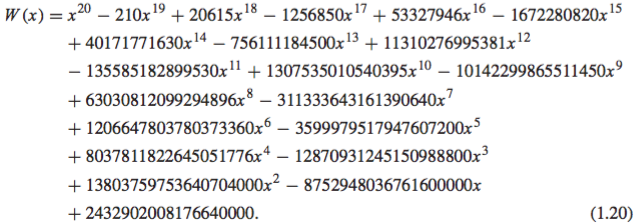
\includegraphics[width=10cm]{figs/1-3-2_Wilkinson_Polynomial-1} 
%\caption{$f(x) = x^3 + x -1$的图像} 
\end{figure}
\end{frame}


\begin{frame}
\frametitle{Wilkinson 多项式}
很容易看到,Wilkinson多项式$W(x)$的根是1到20,但是如果我们利用$W(x)$的展开式进行计算,那么得到的根一般不是这些数值的好的近似。例如如果我们用Matlab中强大的求根命令$fzero$进行求根,以$16$作为初始猜测(注意$16$本身就是这个多项式的一个根),那么求解的结果是
\begin{equation}
x_a \approx 16.01468030580458,
\end{equation}
这个结果只有三位精确的有效数字。我们接下来讨论求根运算的敏感性,尝试解释为什么会出现这样的现象。
\end{frame}


\begin{frame}
\frametitle{求根的敏感性}
如果在输入端的一个小的误差会引起输出端的很大的误差,那么这个问题被称为敏感的。为了定量的讨论问题的敏感性,我们将会引入误差扩大因子和条件数的概念。

\vspace{0.2cm}
为了更好的理解这个问题,我们首先看这样一个问题。如果我们的问题是求$f(x) = 0$的根$r$,但是因为某种原因,我们在输入端产生了一个小的扰动$\epsilon g(x)$。假设$\Delta r$是相对应的输出端的变化(即根的变化),那么我们有
\begin{equation}
f(r + \Delta r) + \epsilon g(r+\Delta r) = 0.
\end{equation}
将$f$和$g$作Taylor展开,得到
\begin{equation}
f(r) + \Delta r f'(r) + \epsilon g(r) + \epsilon (\Delta r) g'(r) + O((\Delta r)^2)  = 0.
\end{equation}
\end{frame}


\begin{frame}
\frametitle{求根的敏感性}
假设$\Delta r$是一个比较小的数,那么$O((\Delta r)^2)$是可以忽略的,从而我们得到
\begin{equation}
(\Delta r) (f'(r) + \epsilon g'(r)) \approx -f(r) - \epsilon g(r) = - \epsilon g(r),
\end{equation}
或者(如果假设$\epsilon$远小于$f'(r)$且$f"(r) \neq 0$)
\begin{equation}
\Delta r \approx \frac{ - \epsilon g(r)}{f'(r) + \epsilon g'(r)} \approx -\epsilon \frac{g(r)}{f'(r)}.
\end{equation}
这个公式称为敏感度公式。
\end{frame}


\begin{frame}
\frametitle{求根的敏感性}
敏感度公式可以帮助我们理解类似于Wilkinson多项式的求根问题为什么比较敏感这个问题。

\vspace{0.2cm}

我们本来要求解的问题是$f(x) = 0$,而$r$是$f(x)$的一个根。因为计算机是有限精度的,我们大致认为由于舍入误差导致我们所求的问题由$f(x) = 0$变成了$f(x) + \epsilon g(x) = 0$。这个时候,如果我们可以理论上求得
$f(x) + \epsilon g(x) = 0$的精确解(相当于不考虑求解过程中的误差),那么这个解也会由原来$f(x) = 0$的解$r$变为$r + \Delta r$。而这个变动$\Delta r$的大小与舍入误差$\epsilon g(x)$的关系正是由敏感度公式
\begin{equation}
\Delta r \approx \frac{ - \epsilon g(r)}{f'(r) + \epsilon g'(r)} \approx -\epsilon \frac{g(r)}{f'(r)}.
\end{equation}
大致给出的。
\end{frame}


\begin{frame}
\frametitle{求根的敏感性}
\begin{example}
估计$P(x) = (x-1)(x-2)(x-3)(x-4)(x-5)(x-6) - 10^{-6}x^7$的最大的根。
\end{example}
令$f(x) = (x-1)(x-2)(x-3)(x-4)(x-5)(x-6)$,$\epsilon = -10^{-6}$而$g(x) = x^{7}$。如果没有$\epsilon g(x)$项,那么最大的根是$r = 6$。现在加上$\epsilon g(x)$项,根据敏感度公式我们得到
\begin{equation}
\Delta r \approx \frac{-\epsilon 6^7}{5!} = -2332.8 \epsilon.
\end{equation}
这说明如果在$f(x)$端产生$10^{-6}$的相对误差,那么在输出端就会产生大约$2000$倍的误差。
\end{frame}


\begin{frame}
\frametitle{求根的敏感性}
由此我们可以估计$P(x)$的根大约是
\begin{equation}
r + \Delta r \approx 6 - 2332.8 \epsilon = 6.0023328.
\end{equation}
而利用$fzero$命令得到的$P(x)$的根为$6.0023268$,两者相差无几。(注意到虽然$fzero$对Wilkinson多项式求根无能为力,但是对于上面给出的$P(x)$求根还是可以比较精确的求出的)。
\end{frame}


\begin{frame}
\frametitle{误差放大因子}
上面的例子中,我们求得的是是向前误差关于向后误差的被放大倍数(上例中如果我们把$r+ \Delta r$作为$x_a$,那么$|\Delta r|$就是向前误差,而$|f(r+\Delta r)| = |\epsilon g(r+\Delta r)|$就是向后误差)。

\vspace{0.2cm}
我们也可以关注相对向前误差关于相对向后误差的倍数。我们令
\begin{equation}
\text{误差放大因子} = \frac{\text{相对向前误差}}{\text{相对向后误差}}.
\end{equation}
根据敏感性公式,我们可以得到
\begin{equation}
\text{误差放大因子}  = \Big|\frac{\frac{\Delta r}{r}}{\frac{\epsilon g(r)}{g(r)}} \Big|
                                = \Big| \frac{\frac{-\epsilon g(r)}{rf'(r)}}{\epsilon} \Big| = \frac{g(r)}{|rf'(r)|} .
\end{equation}
\end{frame}


\begin{frame}
\frametitle{误差放大因子}
注意到这里的相对向后误差的定义为$\frac{|\epsilon g(r)|}{|g(r)|}= |\epsilon|$。我们来解释一下这个定义。

\vspace{0.2cm}
事实上,我们可以将原方程$f(x) = 0$等价的改写为
\begin{equation}
f(x) + g(x) = g(x),
\end{equation}
其解为$x = r$。这时候我们对输入端作一个扰动,将上面的方程变为了
\begin{equation}
f(x) + g(x) = g(x)- \epsilon g(x),
\end{equation}
其解为$x = r+ \Delta r$。这时候求相对向后误差应该是向后误差$|f(r+\Delta r)| = |\epsilon g(r+\Delta r)|$关于方程本身的应该具有的右端项的比值的绝对值,即
\begin{equation}
\text{相对向后误差} =  \frac{|\epsilon g(r+\Delta r)|}{|g(r)|}.
\end{equation}
由于我们认为$\Delta r$相比于$r$较小,因此可以近似的认为$g(r+\Delta r) \approx g(r)$,从而有上面的相对误差的定义。
\end{frame}


\begin{frame}
\frametitle{误差放大因子}
在前面的$P(x)$的例子中,误差扩大倍数就是$\frac{6^7}{5! \times 6} = 388.8$。

\vspace{0.2cm}
我们可以用相同的方法对Wilkinson多项式求根问题进行敏感性分析,并得到其误差放大因子。例如,如果我们考虑$x^{15}$这一项进行一个小的扰动对求$r = 16$这个根的影响就会发现,误差扩大因子大约是$3.8 \times 10^{12}$,这将会让我们失去大约12位的有效数字。
\end{frame}


\begin{frame}
\frametitle{适定性和条件数}
上面求根问题无法得到精确的结果并不是因为我们的计算方法不好(事实上我们可以看到在分析上面求根问题的时候我们并没有考虑算法的影响),而是因为这个问题本身是不适定的。

\vspace{0.2cm}
如果我们定义条件数为一个问题最大的误差放大因子或者在给定条件下最大的误差放大因子(注意我们之前讨论的误差放大因子取决于所求根,即$r$的值,而这里我们可以理解为条件数是我们让$r$取遍所有的根所得到的误差放大因子当中最大的那个),那么一个问题本身条件数很大就称为这个问题是不适定的(ill-conditioned),而如果一个问题的条件数小于1就称为这个问题是适定的(well-conditioned)。条件数与具体的算法无关,是问题本身的性质。

\vspace{0.2cm}
与条件数相对应的一个概念是稳定性。稳定性是指如果算法对于输入端的误差扩大的倍数。

\vspace{0.2cm}
如果一个问题是适定的,而解决这个问题的算法又是稳定的,那么我们可以得到小的向后误差和向前误差。
\end{frame}

%%%%%%%%%%%%%%%%%%%%%%%%%%%%%%%%%%%%%%%%%%



\section{条件数与线性方程组求解}


\begin{frame}
\frametitle{向量范数与误差}
这一部分中,我们考虑线性方程组求解问题的适定性。之前由于我们讨论的是求解非线性方程,所以解是一个实数,因而误差自然是由绝对值来度量的。而线性方程组的解是一个向量,所以我们需要对向量进行度量。

\begin{definition}[无穷范数]
对于一个向量$x = (x_1, \ldots, x_n)$的无穷范数或最大范数的定义是
\begin{equation}
\|x\|_{\infty} = \max_{i = 1, \ldots, n} |x_i|.
\end{equation}
\end{definition}
我们进而有如下定义
\begin{definition}[残量、向前与向后误差]
令$x_a$是线性方程组$Ax = b$的近似解。我们定义方程组的残量为$r = b - Ax_a$。这个方程组的向后误差是$\| b - A x_a\|_{\infty}$,即残量$r$的无穷范数。而这个方程组的向前误差是$\| x_*- x_a\|_{\infty}$,其中$Ax_* = b$。
\end{definition}
\end{frame}


\begin{frame}
\frametitle{线性方程组的误差}
\begin{example}
计算以下方程组
\begin{align}
x_1 + x_2 &= 2 \nonumber \\
1.0001x_1 + x_2 &= 2.0001
\end{align}
在$x = [-1, 3.0001]$处的向前和向后误差。
\end{example}
解上面的线性方程组得到
\begin{align}
x_1 + x_2 &= 2 \nonumber \\
-0.0001 x_2 &= -0.0001
\end{align}
也就是说真解为$[x_1, x_2] = [1,1]$。
\end{frame}


\begin{frame}
\frametitle{线性方程组的误差}
将$x_a$代入方程组得到向后误差为
\begin{align}
b - Ax_a = \left[ \begin{array}{c}
    -0.0001 \\ 0.0001  \end{array} \right].
\end{align}
向前误差为
\begin{align}
x - x_a = \left[ \begin{array}{c}
    2 \\ -2.0001  \end{array} \right].
\end{align}
可以看到,这个问题当中向前误差远大于向后误差,这个问题可以用下面这个图来直观的表示出来
\begin{figure}
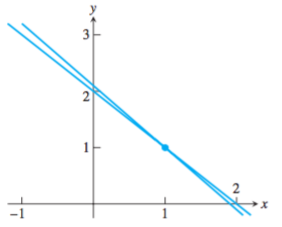
\includegraphics[width=3cm]{figs/2-3-1_Condition_Number-1} 
%\caption{$f(x) = x^3 + x -1$的图像} 
\end{figure}
\end{frame}


\begin{frame}
\frametitle{相对误差}
为了与之前的讨论向对应,我们定义$Ax = b$在$x_a$处的相对向后误差为
\begin{equation}
\frac{\|r\|_{\infty}}{\|b\|_{\infty}},
\end{equation}
其中$r = b - Ax_a$。相对向前误差为
\begin{equation}
\frac{\|x_*-x_a\|_{\infty}}{\|x_*\|_{\infty}},
\end{equation}
其中$x_*$为$Ax = b$的真解。则误差扩大因子为
\begin{equation}
\text{误差扩大因子} = \frac{\frac{\|x_*-x_a\|_{\infty}}{\|x_*\|_{\infty}}}{\frac{\|r\|_{\infty}}{\|b\|_{\infty}}}.
\end{equation}
例如之前的例子中相对向后误差为$0.005\%$而相对向前误差为$200\%$,则误差扩大因子为$40004.0001$.
\end{frame}


\begin{frame}
\frametitle{矩阵范数}
为了刻画条件数,我们需要用到矩阵范数,我们定义一个矩阵$A$的无穷范数为
\begin{equation}
\|A\|_{\infty} = \max_{i = 1, \ldots, n} \sum_{j = 1}^{n} |a_{ij}|.
\end{equation}
事实上,我们可以证明
\begin{equation}
\|A\|_{\infty} = \max_{x \in \R^n} \frac{\|Ax\|}{\|x\|}.
\end{equation}
\end{frame}


\begin{frame}
\frametitle{条件数}
与之前的定义类似,一个线性方程组的条件数与其系数矩阵的性质相对应,就是所有可能的误差扩大因子中最大的一个。我们可以证明如下定理
\begin{theorem}
一个$n \times n$的矩阵$A$的条件数为
\begin{equation}
\text{{\rm{cond}}}(A) = \|A\|_\infty \|A^{-1}\|_\infty
\end{equation}
\end{theorem}
\begin{proof}
\ \\
\ \\
\ \\
\ \\
\end{proof}
\end{frame}


\begin{frame}
\frametitle{条件数}
\begin{example}
求矩阵
\begin{equation}
A =  \left[ \begin{array}{cc}
     1    &  1 \\
      1.0001   &  1                
            \end{array} \right] .
\end{equation}
的条件数。
\end{example}
容易求得$\|A \|_\infty = 2.0001$。同时
\begin{equation}
A^-1 =  \left[ \begin{array}{cc}
     -10000    &  10000 \\
      10001   &  -10000                
            \end{array} \right] .
\end{equation}
因此$\|A^{-1}\| = 20001$。因此$A$的条件数是
\begin{equation}
\text{{\rm{cond}}}(A) = (2.0001)(20001) = 40004.0001.
\end{equation}
\end{frame}
%%%%%%%%%%%%%%%%%%%%%%%%%%%%%%%%%%%%%%%%%%

\begin{frame}
\frametitle{课后阅读及作业}
[NA] 第1章 1.3;第2章 2.3.1\\
作业:[NA] 第1章1.3: 1,5,8;第2章 2.3: 1,2,5。


\end{frame}

\end{document}

